%For a Tutorial, how to install Latex and using it with vscode, follow this Website:
%https://medium.com/@erencanbulut/boost-your-latex-workflow-with-vs-code-and-github-f346b74677be

\documentclass[12pt,bibtotoc]{article}% Legt die Dokumentenklasse als Artikel mit Schriftgröße 12pt fest und fügt das Literaturverzeichnis zum Inhaltsverzeichnis hinzu.
\usepackage[table]{xcolor}% Ermöglicht farbige Gestaltung von Tabellenzellen und anderen Elementen.
\usepackage[ngerman]{babel} % Für Silbentrennung
\usepackage[utf8]{inputenc} % Um Umlaute und Sonderzeichen nutzen zu können
\usepackage[a4paper,
lmargin={2cm},
rmargin={2cm},
tmargin={2cm},
bmargin={3cm}]{geometry} % Für das Layout
\usepackage{setspace} % Für den Zeilenabstand
\setstretch{1.25}% Setzt den Zeilenabstand auf das 1,25-fache, um den Text lesbarer zu machen.
\usepackage{graphicx} % Um Bilder einzufügen
\usepackage{wrapfig} % Um Bilder im Fließtext einzubinden
\usepackage{csquotes} % Um Text in Anführungsstriche zu setzen
\usepackage{mathptmx} % Ähnlich zu Times New Roman
\usepackage{fancyhdr} % Um den Header einzufügen
\usepackage{pdfpages} % Um die Titelseite einbinden
\usepackage{hyperref} % Um Verlinkungen einfügen
\usepackage{acronym} % Um Akronyme zu definieren
\usepackage{textcomp} % Um spezielle Zeichen verwenden zu können (z.B. °, µ)
\usepackage{subcaption} % Um mehrere Bilder zusammen einzustellen und Links zu Abbildungen zu korrigieren
\usepackage{float}% Ermöglicht die präzise Platzierung von Gleitobjekten (wie Tabellen und Abbildungen) im Dokument.
\usepackage{placeins}% Verhindert, dass Gleitobjekte (z.B. Tabellen oder Abbildungen) über bestimmte Stellen im Text hinausrutschen, indem \FloatBarrier verwendet werden kann.
\usepackage{cleveref} %für Querverweise auf Kapitel: see section \cref{Kapitelname}

%Anpassung für itemize:
\usepackage{enumitem} % Ermöglicht die Anpassung von Listenformatierungen, z.B. bei Aufzählungen.
\setlist[itemize]{itemsep=0pt, topsep=0pt, leftmargin=1.5em} % Setzt den Abstand zwischen Listenelementen auf 0 und reduziert den Einzug der Aufzählung.


\floatplacement{figure}{H} % Erzwingt, dass Abbildungen genau an der Stelle im Text erscheinen, an der sie definiert sind (H = here).

\usepackage[backend=bibtex, citestyle=ieee]{biblatex} % Um Literatur einzufügen

\bibliography{Quellenverzeichnis} % Verweist auf die Datei 'Quellenverzeichnis.bib' für die Literaturangaben im Dokument.

\pagestyle{fancy} % Aktiviert benutzerdefinierte Kopf- und Fußzeilen im Dokument.
\fancyhf{} % Löscht alle Voreinstellungen für Kopf- und Fußzeilen.
\setlength\headheight{59.76491pt} % Passt die Höhe der Kopfzeile an die eingefügte Grafik an.
\renewcommand{\headrulewidth}{0pt} % Entfernt die Standardlinie unter der Kopfzeile.

%Falls es sich eher um eine Hausarbeit als um eine Transferleistung handelt, einfach stattdessen folgendes Bild einhängen: Resources/header_withoutTransfer.png
\chead{
\includegraphics[width=\textwidth]{Resources/header.png}} % Fügt eine Grafik als zentrierten Header in die Kopfzeile ein.

\cfoot{\thepage} % Setzt die Seitenzahl zentriert in die Fußzeile.

\newcounter{romanBeginningEnd} % Um Römische Seitenzahl zu speichern

% Sektionen referenzen anpassen
\addto\extrasngerman{%
	\renewcommand{\sectionautorefname}{siehe} % Ändert die automatische Referenzbezeichnung für 'section' auf "siehe".
	\let\subsectionautorefname\sectionautorefname % Setzt die automatische Referenzbezeichnung für 'subsection' auf die gleiche wie für 'section'.
	\let\subsubsectionautorefname\sectionautorefname % Setzt die automatische Referenzbezeichnung für 'subsubsection' auf die gleiche wie für 'section'.
}




\begin{document}
    \pagenumbering{gobble}
    \newpage




\definecolor{color_30879}{rgb}{0,0.12549,0.376471}
\vspace{20mm}
\noindent
{\fontsize{15.96}{1}\usefont{T1}{cmr}{m}{n}\selectfont\color{color_30879}Transferleistung Theorie/Praxis  }\\ 
{\fontsize{15.96}{1}\usefont{T1}{cmr}{m}{n}\selectfont\color{color_30879}Nr. 2} 

\vspace{15mm}



\begin{center}
\begin{tabular}{ |>{\columncolor{color_30879}}p{1.6in} | p{4.4in}| } 
 \hline
 \textcolor{white}{Martrikelnummer:} & 12657 \\[0.2in]
 \hline
 \textcolor{white}{Freigegebenes Thema:} & Wie kann Knk das optimale Hosting-Modell auswählen, das den spezifischen Anforderungen und Zielen des Kunden entspricht, um Kosten zu optimieren, Flexibilität sicherzustellen und gleichzeitig Sicherheits- und Compliance-Anforderungen gerecht zu werden? \\ [1in]
 \hline
 \textcolor{white}{Studiengang, Zenturie:} & Wirtschaftsinformatik, I22c \\ [0.2in]
 \hline
\end{tabular}
\end{center}

	%\includepdf[pages=-]{Resources/cover}
	
	\setcounter{page}{1} % Römische Seitenzahlen
	\pagenumbering{Roman}
	
	\tableofcontents %Inhaltsverzeichnis
	\newpage
	
	\setcounter{secnumdepth}{0} % Keine Numerierung von Überschriften
	\clearpage
	\phantomsection
	\addcontentsline{toc}{section}{\listfigurename} % Abbildungsverzeichnis im Inhaltsverzeichnis anzeigen
	\listoffigures
	\clearpage
	\phantomsection
	%\addcontentsline{toc}{section}{\listtablename} % Tabellenverzeichnis im Inhaltsverzeichnis anzeigen
	%\listoftables
	\newpage
	\section{Abkürzungsverzeichnis}

	% Abkürzungen
	\begin{acronym}[LängsteAbkürzung] % Für Formatierung längste Abkürzung eintragen
	% Beispiel:
	\acro{ac:Label}[MA]{Mitarbeiter}
	\end{acronym}
	\newpage
	
	\setcounter{secnumdepth}{3} % Überschriften wieder normal numerieren
	
	\setcounter{romanBeginningEnd}{\the\value{page}} % Speichern der römischen Seitenzahl
	\setcounter{page}{1} % Mit Arabischen Seitenzahlen wieder bei 1 anfangen
	\pagenumbering{arabic}
	
	% ###############################################################
	% Tipps und Tricks:
	%\section{Begriffserklärung}
	%Beispieltext
	%\subsection{Was ist der Fachkräftemangel}
	%\newpage
	
	
	%\begin{figure}[h!]
		%\includegraphics[keepaspectratio,width=\textwidth,height=\textheight]{statistaEntwicklungFachkraefteindex.png} \renewcommand{\figurename}{Abb.}
		%\caption{\small Entwicklung des Fachkr{\"a}fteindex in Deutschland vom 1. Quartal 2015 bis zum 4. Quartal 2022; Hays über Statista, 2023}
	%\end{figure}

	% Zitieren:
	%\cite{BeispielCite} BeispielCite = Name einer Zitation aus dem Quellenverzeichnis
	
	%\newpage

	% Einbinden einer figure:
	% \begin{figure}[H] %Nutzung von Cloud Computing in Unternehmen in Deutschland in den Jahren 2011 bis 2022
	% 	\centering
	% 	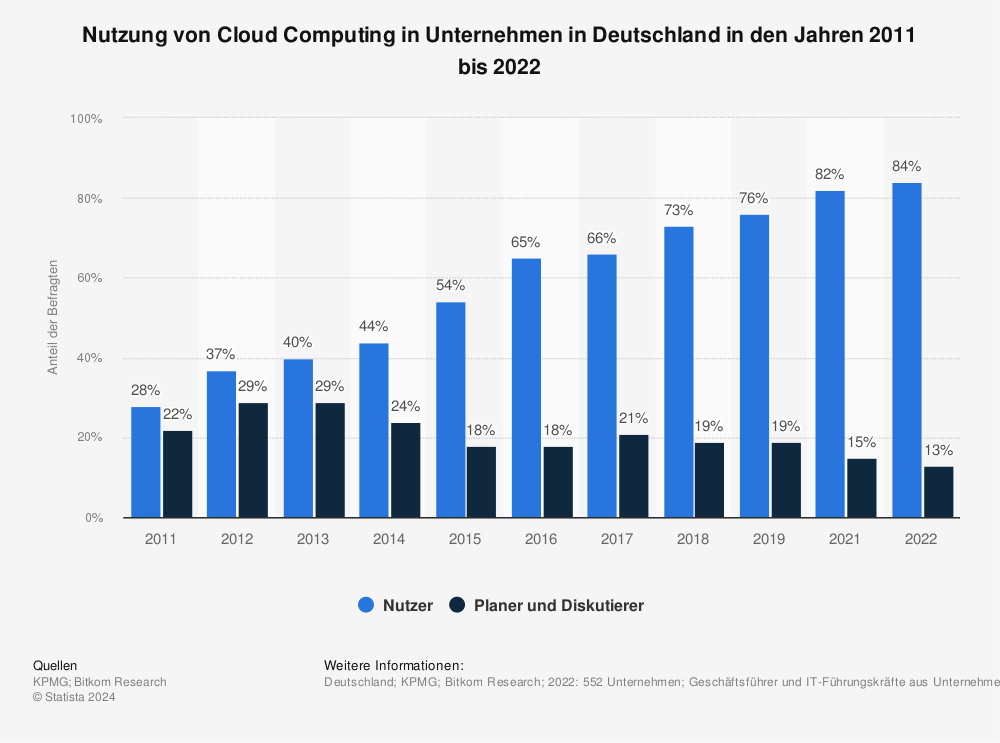
\includegraphics[keepaspectratio,width=\textwidth,height=\textheight]{"Content/Pictures/Nutzung von Cloud Computing in Unternehmen in Deutschland in den Jahren 2011 bis 2022.png"} 
	% 	\renewcommand{\figurename}{Abb.}
	% 	\caption{\small Nutzung von Cloud Computing in Unternehmen in Deutschland in den Jahren 2011 bis 2022}
	% \end{figure}
	
	%(\cite{Oelsnitz.2023}, Seite 4-5)

	%\begin{quote}
	%	,,Der aktuelle Wandel in Wirtschaft und Gesellschaft führt zu Umw{\"a}lzungen in einem bislang nicht gekannten Ausmaß. Strukturen, Prozesse, Aufgabenzuschnitte ver{\"a}ndern sich
	%	grundlegend – und dies in nahezu allen Branchen und Gesch{\"a}ftsbereichen.''\newline (\cite{Longmu.2021}, Seite 3)
	%\end{quote} --> Sowas wie {\"a} statt ä, muss nicht mehr gemacht werden. Dafür wurde package installiert.

	%################################################################
	%Ab hier Inalt

	% Inhalt ende
	% ###############################################################

	\newpage % Beginnt eine neue Seite.
	\pagenumbering{Roman} % Setzt die Seitenzahlen auf römische Zahlen.
	\setcounter{page}{\theromanBeginningEnd} % Setzt den Seitenzähler auf den angegebenen römischen Wert fort.
	\setcounter{secnumdepth}{0} % Deaktiviert die Nummerierung der Überschriften.
	\section{Quellenverzeichnis} % Erzeugt eine neue Sektion für das Quellenverzeichnis.
	%\includepdf[pages=-]{Resources/cover} % Kommentiert: Fügt eine PDF-Datei als Deckblatt ein (alle Seiten). (wusste nicht ob das noch irgendwann mal gebracht wird, deswegen sicherheitshalber drinnen gelassen)
	\setcounter{secnumdepth}{3} % Aktiviert die Nummerierung von Überschriften bis hinunter zu Subsubsections (für den Anhang).
	\printbibliography[heading=none] % Gibt das Literaturverzeichnis aus, ohne eine Überschrift.
	\newpage % Beginnt eine neue Seite.
	\appendix % Kennzeichnet den Beginn des Anhangs.
	\clearpage % Erzwingt das Ende der aktuellen Seite und beginnt eine neue.
	\addcontentsline{toc}{part}{Anhang} % Fügt den Anhang zum Inhaltsverzeichnis hinzu.
	%\includepdf[pages=-,picturecommand*={\label{MEINPDFDOKUMENT}}]{Content/Documents/PDF/21.08.2024 Experteninterview mit (unterschrieben und korrigiert).pdf} % Fügt ein externes PDF-Dokument ein und setzt ein Label.

\end{document}